%% Example of a LaTeX source file for a COLING-2012 submission
%% last updated: July 10, 2012
%% Optional instructions for authors within the tex file are provided as comments and start with 'for authors:...'
\documentclass[10pt,a5paper,twoside]{article}
\usepackage{coling2012}

\title{Rule-based Machine Translation between Indonesian and Malaysian}

%for authors: in case of more than four author names ref. to commented line below 
%\author{$Annie~SMITH^{1, 2}~~~LI~Xiao Dong^{1, 3}$\\$~~~Third~Author^{1, 2}~~~Fourth~Author^{1, 3}~~~ Fifth~Author^{2, 3}$\\
\author{$Raymond~Hendy~Susanto^{1}$\\
{\small  	(1) Department of Computer Science, National University of Singapore\\ 
 		%(2) INSTITUTE\_2, address 2\\
		%(3) INSTITUTE\_3, address 3\\
  \texttt{raymondhs@nus.edu.sg} \\ 
}}

\begin{document}
\maketitle
%% The first mandatory ABSTRACT (\abstractEn) section below is for the English language
\abstractEn{  %ABSTRACT}{
We describe the development of a bidirectional machine translation system between Indonesian and Malaysian, two closely related Austronesian languages widely spoken by 180 million speakers around the world. The system is based on the re-use of free and publicly available resources, such as the Apertium machine translation platform and Wikipedia. We also present our approaches to overcome the data scarcity problems in both languages by exploiting the morphology similarities between the two.}

%for authors: the line below is for instruction purposes and can be commented
%\textbf{AT SUBMISSION TIME, PLEASE ANONYMISE everywhere, REPLACING NAMES BY DUMMIES LIKE John DOE\_1, Jack DOE\_2.}

%for authors: the abstract section below is optional and can be commented otherwise
%% The second ABSTRACT (\abstractOL) given below is for the optional language
% \abstractOL{ %TITLE AND ABSTRACT IN ANOTHER LANGUAGE, $L_{2}$ (OPTIONAL, AND ON SAME PAGE)}{
% \\\\
% {\centering{{\Large{\textbf{Translation in $L_{2}$ of the article title}}} (if option used):14pt, bold,centered}}\\\\
% The translation of the title and abstract in another language $L_{2}$ is optional.  If the title is translated, the abstract must also be translated, as exactly as possible. In that case, put an abstract in $L_{2}$ (maximum 170 words as translation expands text length) here.\\\\
% Apart from enhancing visibility in one’s own national scientific communities, these parallel abstracts might be the seed for a multilingual natural parallel corpus in computational linguistics.
% Tantus est igitur innatus in nobis cognitionis amor et scientiae ut nemo dubitare possit quin ad eas res hominum natura nullo emolumento invitata rapiatur. Videmusne ut pueri ne verberibus quidem a contemplandis rebus perquirendisque deterreantur ? Ut pulsi recurrant? Ut aliquid scire se gaudeant ? Ut id aliis narrare gestiant ? Ut pompa, ludis atque eius modi spectaculis teneantur ob eamque rem vel famem et sitim perferant ? Quid vero ? 
% }

%%-------------
%for authors: if only English language option is chosen comment the \abstractOL section above and use \keywordsEn below 
%for authors: else use add title and abstract to \abstractOL section above and use \keywordsOL below (case-sensitive commands)

%for authors: for keywords section either use \keywordsEn OR \keywordsOL below as relevant
%Example for English only keywords list
\keywordsEn{machine translation, Malay languages, morphology}

%Example for English + optional language keywords list
%\keywordsOL{Here a list of keywords in English}
%{Here a list of keywords in $L_{2}$ (if option used)}
%%--------------

\newpage
\section{Introduction}

\section{System}
The system is based on the Apertium machine translation platform \citep{apertium/2011}.\footnote{\url{http://www.apertium.org/}} The platform was originally aimed at the Romance languages of the Iberian peninsula, but has also been adapted for other, more distantly related language pairs. The whole platform, both programs and data, are licensed under the Free Software Foundation's General Public Licence\footnote{\url{http://www.fsf.org/licensing/licenses/gpl.html}} (GPL) and all the software and data for the 33 supported language pairs (and the other pairs being worked on) is available for download from the project website.

\subsection{Architecture of the system}

\begin{figure*}[htbp]
\begin{center}
 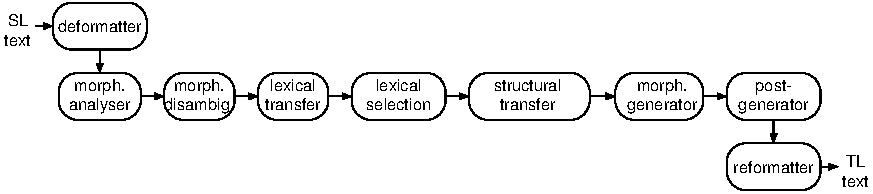
\includegraphics[width=0.8\textwidth]{architecture.pdf}
\end{center}
\caption{The pipeline architecture of the Apertium system.}
\label{fig:modules}
\end{figure*}

The Apertium translation engine consists of a Unix-style \emph{pipeline} or
\emph{assembly line} with the following modules (see Fig.~\ref{fig:modules}):  
\begin{itemize}
\item A \emph{deformatter} which encapsulates the format information
 in the input as \emph{superblanks} that will then be seen
 as blanks between words by the other modules.
\item A \emph{morphological analyser} which segments the text in
  surface forms (SF) (\emph{words}, or, where detected, multi-word lexical
  units or MWLUs) and for each, delivers one or more \emph{lexical
    forms} (LF) consisting of \emph{lemma}, \emph{lexical category} and
  morphological information. 
\item A \emph{morphological disambiguator} (constraint grammar) which chooses, using linguistic rules
  the most adequate sequence of morphological analyses for an ambiguous sentence. 
\item A \emph{lexical transfer} module which reads each SL LF 
  and delivers the corresponding target-language (TL) LF
  by looking it up in a bilingual dictionary encoded as an FST
  compiled from the corresponding XML file. The lexical transfer module may
  return more than one TL LF for a single SL LF.
\item A \emph{lexical selection} module which chooses, based on context 
  rules the most adequate translation of ambiguous source language LFs.
\item A \emph{structural transfer} module which
    performs local syntactic operations, is compiled from XML files containing rules that 
    associate an \emph{action} to each defined LF \emph{pattern}. Patterns are applied left-to-right, and the 
    longest matching pattern is always selected.
\item A \emph{morphological generator} which delivers a TL SF
 for each TL LF, by suitably inflecting it. 
\item A \emph{reformatter} which de-encapsulates any format
  information.
\end{itemize}

\subsection{Morphological transducers}
There is one publicly available morphological tool for Indonesian, namely MorphInd \citep{larasati2011indonesian}. However, MorphInd is only designed for analysis, while we wanted the dictionary to be able to be used for both morphological analysis and generation. Moreover, there are rarely linguistic resources and tools available for Malaysian language. \citet{Baldwin06opensource} has developed a free/open-source lemmatiser for Malay, but this does not meet our need either since we wanted to include other important morphological information in our Malaysian transducer, such as parts of speech and affixes. Thus, we decided to build the morphological transducers from scratch.

Similar to most Apertium language pairs, the morphological transducers for both Indonesian and Malaysian are constructed using \emph{lttoolbox}, a toolbox for morphological analysis and generation that is available under free/open-source licence. The monolingual dictionary for each language is provided as XML-formatted entries, which is then compiled into a fast finite state transducers using the toolbox.

\subsubsection{Indonesian morphological transducer}
The words were added semi-automatically to the Indonesian morphological analyser based on frequency, with the most frequent words being added first. The frequency list was taken from a database dump of the Indonesian Wikipedia. For each word in the frequency list, we obtained its lemma and part of speech information from Kateglo\footnote{\url{http://kateglo.bahtera.org/}}, an online Indonesian dictionary with over 70,000 entries licensed under CC BY-SA 3.0\footnote{\url{http://creativecommons.org/licenses/by-sa/3.0/}}. Since we also wanted to include affix information in our analyser, we wrote a rule-based morpheme separator to decompose a given Indonesian surface form into their constituent morphemes, also by making use of the lemma information from Kateglo. Moreover, closed classes (e.g. pronouns, conjunctions) were added by hand.

\subsubsection{Malaysian morphological transducer}
A frequency list for Malaysian was also created based on a database dump of the Malaysian Wikipedia. Unlike Indonesian, we barely found a comprehensive Malaysian dictionary with adequate morphological information, such as lemma and part of speech. Hence, the Malaysian analyser was built using the two strategies below.

First, Malaysian words that also exist as an Indonesian word were assumed to share the same morphological information (i.e. the same lemma and part of speech), and added automatically to the analyser. Although this method may introduce a number of false friends (e.g. \emph{polisi} means `policy' in Malay but `police' in Indonesian), the benefit outweighs the risk since there is huge overlap in the lexicons of the two languages. Moreover, most of these false friends usually belong to the same part of speech.

Second, we also added Malaysian words which appear in our bilingual lexicon. Since every entry in a bilingual lexicon is a pair of words with the same meaning, we can assume that these words also belong to the same part of speech most of the time. Our approaches to building the bilingual dictionary are presented in the following section.

\subsection{Bilingual dictionary}
There is no freely available bilingual dictionary between Indonesian and Malaysian, so we had to build the dictionary from scratch. At the moment, the bilingual dictionary contains 12,142 entries, which was developed in several ways described below.

First, most of the entries were added using automatic word alignments. We created an Indonesian-Malaysian parallel corpus by translating many articles taken from Malaysian Wikipedia. The translation process is mostly automatic, with the help of existing Malaysian-Indonesian machine translation system such as Google Translate.\footnote{\url{http://translate.google.com/}}

Next the Wikipedia corpus is tagged using our morphological analyser, and word alignments were created by running \texttt{Giza++} \citep{Och2003align} on the tagged corpus. We fed the probabilistic dictionary into the \texttt{ReTraTos} toolbox \citep{Caseli2006retratos}, which extracts both phrases and single-word translations from alignments, and converts them into Apertium translation entries. The \texttt{ReTraTos} method gave us about 12,000 translation entries, but also required a manual check due the amount of noise in the resulting data.

Finally, some entries were added manually, which included closed classes and words that frequently appeared in Wikipedia but were not yet added to the bilingual dictionary.
% section 2
\section{Main content of the paper (in English)}
% subsection 2.1
\subsection{General information}
This template continues as if the "other language" option had been chosen, meaning that the article proper, in English, begins on page 4. Its length corresponds to that of a short paper.

USUAL but IMPORTANT: papers must conform to the official COLING-2012 style guidelines (downloadable from the website).

Submission and reviewing will be on-line, managed by the START system. The only accepted format for submitted papers is PDF. Supplementary material, if any, in the form of tools or resources, must be in the form of a single .zip or a .tgz archive file with a maximum size of 10MB; otherwise there are no constraints on its format. Submissions, together with all supplementary material, must be uploaded on the START system by the submission deadlines; submissions after that time will not be reviewed.

To minimize network congestion, we request authors to upload their submissions as early as possible (especially if they contain large supplementary material files). Improved versions of the submissions may be uploaded until the deadline.

Submissions must be in the format described in this template. If for some reason you have a problem producing this format, please contact organisers as early as possible. Organisers reserve the right not to publish papers not conforming to the required format.

On acceptance of a submission, precise instructions will be given on how to send the camera ready version, and in some cases with required modifications. Camera ready versions not conforming to programme committee’s improvement requests will be considered as unsent, and hence will not be presented at the conference and will not be included in the proceedings.
% subsection 2.2
\subsection{More on the format of submissions}
Since several years, scientific conferences have been distributing proceedings on electronic media to avoid producing printed versions. Printed versions are given to only those participants who explicitly request and pay for them. Most participants get the proceedings on a CD or on a USB key. That is a very good idea, but the drawback is that very few participants manage to read more than a small number of papers, typically less than 1/10th or 1/20th of the number available in the proceedings. The main reason seems to be that is it very awkward to read traditional A4 sized portrait double-column articles on usual laptop screens. 

The recent JEP-TALN-RECITAL-2012 conferences have successfully addressed that problem by proposing a template that is optimised for reading on PC screens. COLING-2012 and associated events propose to use it, with the option of using the Times New Roman font for authors having problems with installing the slightly better fonts Charter, Charis, or Georgia. 

%% below commented section for testing font sizes ---------
%\\{\small text with small style}\\
%line formatted with default font style equal normalsize (and is10pt; as defined in the \documentclass)\\
%{\normalsize text with normalsize style, \textbf {More on the format of submissions}}\\
%{\large text with large style, \textbf {More on the format of submissions}}\\
%{\Large text with Large style, \textbf {More on the format of submissions}}\\
%% end font size testing -----------
-
% 2.2.1
\subsubsection{Document format\& character fonts}
\emph{Submissions will be in PDF, with page dimensions of 150 mm x 210 mm, and margins of 5 mm on all sides.} That corresponds to A5 (148.2 mm x 209.9 mm) with 4.1 mm horizontal margins and 5 mm vertical margins.  To get the same layout on an A4 format while preparing a submission, choose A4 and put the margins at 35 mm (horizontal) and 48.3 mm (vertical).
\newpage
\emph{No header or footer should be present in submissions.}

The \emph{preferred fonts} have been chosen because they are optimised for reading on screen while being elegant in print. If possible, submissions prepared with LaTeX should use the \emph{Charter (Bitstream)} font. Users of Word or LibreOffice should use an equivalent font, namely (in order of preference):
\begin{compactenum}
\item\emph{Charter} (via Bitstream), available on most Linux and in LaTeX \emph{texlive} installations.
\item\emph{Charis SIL} (via SIL). It is an extension of the Charter font, and is available at \href{http://scripts.sil.org/cms/scripts/page.php?item_id=CharisSIL_download}
{http://scripts.sil.org/cms/scripts/page.php?item\_id=CharisSIL\_download}); 
\item\emph{Georgia.} This font is included  in MS Word by default.
\end{compactenum} 
If authors encounter problems in installing one of the preferred fonts, they should use Times New Roman (available in all platforms) as default font, with the same point sizes.

\emph{The body of the text should be in size 10pt, the titles in bold 11pt for levels 1 \& 2, and 10pt from level 3 onwards.}
%2.2.2
\subsubsection{Pages and paragraphs}
Paragraphs use single spacing and are justified left and right. They are not indented, but are separated by a half-line vertical space (6pt above and below).

The first page contains only the title, the names and affiliations of authors, the abstract(s) and the keywords (see page 1 of this template).

The body of the paper, including the introduction, begins on page 4 if a condensed (2-page) synopsis in another language L$_{2}$ is included, and on page 2 otherwise. 

A LaTeX stylesheet, a Word template, and an ODT template are available on the COLING-2012 website. Submissions will be handled interactively under SoftConf. 
%2.2.3
\subsubsection{Submission sizes}
Here are the length limits according to the type of submission. "Any number of reference pages" means that pages used for bibliographical and Internet references are not counted in the page number limits. However, it stands to reason that reviewers will accept only reasonable sizes.\\\\\\
\begin{tabular}{|l|l|l|}
\hline
full papers & 14 A5 pages with any number of reference pages & Oral presentation\\
\hline
short papers & 8 A5 pages with any number of reference pages & Poster presentation\\
\hline
demo papers & 6 A5 pages with any number of reference pages & Demonstration\\
\hline
\end{tabular}\\

Papers are in English. However, if an author so wishes s/he may add elements in another language (L$_{2}$): a title, an abstract and keywords on the first page, and 2 pages (a synopsis) in L$_{2}$, beginning on page 2. Such papers will have 14+2 (or 8+2, or 6+2) pages, plus any number of pages for reference. 
%2.3
\subsection{Other formatting elements}
%2.3.1	
\subsubsection{Lists}
Here is a bulleted list, where each element begins with an independent sentence (capitalized).
\begin{compactitem}
\item Its lines are separated by less vertical space than normal paragraphs.
\item We don’t add space between paragraphs of that same style.
\end{compactitem}

Here is a numbered list of items that are parts of an outside sentence. Take care to:
\begin{compactenum}
\item restart the numbering and get the numbers consecutive. 
\item not to capitalize the initial letter of such items.
\end{compactenum}
%2.3.2
\subsubsection{Figures and tables}
Figures and tables will be centered on the page, with a caption underneath. The caption will contain the keyword \textsc{Figure} or \textsc{Table} in small capitals, followed by the number of the figure or table. Numbers in each category are independent. Examples appear in this template. Equations and formulae may appear in line or centered on the page, without captions. A reference number may appear to the right of a formula or an equation.

\begin{table}[!h]
\setcounter{table}{0}
\centering
	\begin{tabular}{|c|p{5cm}|}
	\hline
	A table&\\
	\hline
	&The table is centered. Its cells may be optionally centered. Avoid full justification leading to very long horizontal spaces.\\
	\hline
	\end{tabular}
\caption{A table caption appears under it.}\label{Table}
\end{table}
%2.3.3
\subsubsection{Notes and references}
Footnotes\footnote{Here is one!} can be used.

References to the bibliography, for example \cite{Bernhard07}, are formatted with the APA style (see \href{http://www.apastyle.org/}{http://www.apastyle.org/}). It is available in all the LaTeX installations based on \emph{texlive} and on CTAN.

Users of Word or LibreOffice are encouraged to follow this style as much as possible when using their bibliography management tool (Mendeley, Zotero or Endnote). They can refer to the example below. Authors citing online references (URLs) should include the creation date in the reference.

The rest of this document only illustrates the format described above.

Tantus est igitur innatus in nobis cognitionis amor et scientiae ut nemo dubitare possit quin ad eas res hominum natura nullo emolumento invitata rapiatur. Videmusne ut pueri ne verberibus quidem a contemplandis rebus perquirendisque deterreantur ? Ut pulsi recurrant? Ut aliquid scire se gaudeant ? Ut id aliis narrare gestiant ? Ut pompa, ludis atque eius modi spectaculis teneantur ob eamque rem vel famem et sitim perferant ? Quid vero ? Qui ingeniis studiis atque artibus delectantur, nonne videmus eos nec valetudinis nec rei familiaris habere rationem omniaque perpeti ipsa cognitione et scientia captos et cum maximis curis et laboribus compensare eam quam ex discendo capiant voluptatem ?
\newpage
\begin{figure}[htbp] 
\begin{center}
\includegraphics[scale=0.70]{coling_logo.jpg}
\caption{An image used as a figure: It is a good idea to put each figure in a table cell to avoid (in Word) problems with anchored or floating figures.}
\label{image} %
\end{center} 
\end{figure} %
Omne hoc tempus inter pugillares ac libellos iucundissima quiete transmisi. "Quem ad modum, inquis, in urbe potuisti ?"

Circenses erant, quo genere spectaculi ne levissime quidem teneor. nihil novum, nihil varium, nihil quod non semel spectasse sufficiat. Quo magis miror tot milia virorum tam pueriliter identidem cupere currentis equos, insistentis curribus homines videre.

Si tamen aut velocitate equorum aut hominum arte traherentur, esset ratio non nulla; nunc favent panno, pannum amant, et, si in ipso cursu medioque certamine hic color illuc, ille huc transferatur, studium favorque transibit, et repente agitatores illos, equos illos, quos procul noscitant, quorum clamitant nomina, relinquent. Tanta gratia, tanta auctoritas in una vilissima tunica, mitto apud volgus, quod vilius tunica, sed apud quosdam graves homines; quos ego cum recordor in re inani, frigida, assidua tam insatiabiliter desidere, capio aliquam voluptatem, quod hac voluptate non capior.

Ac per hos dies libentissime otium meum in litteris colloco, quos alii otiosissimis occupationibus perdunt. Vale. (PLINE Junior, Letters, IX, 6.) 
\begin{figure}[htbp]
\begin{center} 
\includegraphics[scale=0.4]{illustration2.jpg} 
\caption{It is not advised to use Word directly to generate drawings. Use another tool (even Powerpoint) and insert the resulting image (at least 300 DPI or in vectorised format).}
\label{figure}
\end{center}
\end{figure} 

%3
\section{Title of a section}
Rem atrocem nec tantum epistola dignam Larcius Macedo, vir praetorius, a servis suis passus est, superbus alioqui dominus et saevus et qui servisse patrem suum parum, immo nimium meminisset. Lavabatur in villa Formiana; repente eum servi circumsistunt, alius fauces invadit, alius os verberat, alius pectus et ventrem atque etiam, foedum dictu, verenda contundit; et, cum exanimem putarent, abiciunt in fervens pavimentum, ut experirentur an viveret. 

Ille, sive quia non sentiebat, sive quia non sentire se simulabat, immobilis et extentus fidem peractae mortis implevit. Tum demum quasi aestu solutus effertur; excipiunt servi fideliores, concubinae cum ululatu et clamore concurrunt. Ita et vocibus excitatus et recreatus loci frigore, sublatis oculis agitatoque corpore vivere se - et iam tutum erat - confitetur. \\
\newpage
Diffugiunt servi quorum magna pars comprehensa est, ceteri requiruntur; ipse paucis diebus aegre focilatus non sine ultionis solacio decessit, ita vivus vindicatus ut occisi solent. (PLINE, Letters, III, 14.)
%3.1	
\subsection{Title of a subsection}
Miles cum oboediens potestati, sub qua legitime constitutus est, hominem occidit, nulla civitatis suae lege reus est homicidii; immo, nisi fecerit, reus est imperii deserti atque contempti. Quod si sua sponte atque auctoritate fecisset, in crimen effusi humani sanguinis incidisset. Itaque unde punitur si fecit iniussus, inde punietur nisi fecerit iussus. Quod si ita est, iubente imperatore, quanto magis, iubente creatore ! 
%3.1.1
\subsubsection{Title of a subsubsection}
Qui ergo audit non licere se occidere, faciat, si iussit cuius non licet iussa contemnere; tantummodo videat utrum divina iussio nullo nutet incerto... Hoc dicimus, hoc asserimus, hoc modis omnibus approbamus neminem spontaneam mortem sibi inferre debere velut fugiendo molestias temporales, ne incidat in perpetuas. (Sanctus Augustinus.)

\section*{Conclusion and perspectives (not numbered, use style “Heading1”)} %  not numbered
This section should better not be numbered (style “Heading1” inherits from “Heading 1”).
\section*{Acknowledgments (not numbered, use style Heading1)}
Optional section. If some named entities may lead to authors identification, please anonymize them.	\\
Thanks to Gilles S\'erasset for having kindly shared with us the templates he devised for TALN-JEP-RECITAL-2012. 

%'apalike-fr' style below applies smallcaps style on author names
%in order to apply 'apalike-fr' the babel package must be given [frenchb] option instead of [english]
% \usepackage[frenchb]{babel} also causes title "References" to render with French accents like "R\'ef\'erences"
%\bibliographystyle{apalike-fr}

%'apa' style does not apply "smallcaps style" on author names and goes with the [english] option in the babel package

\bibliographystyle{apa}

\bibliography{id-ms.coling2012}

\end{document}
